\chapter{Mathematische Grundlagen der RSA-Verschlüsselung}

% ✓Definition und ✓Anwendungsbeispiel + Wofür (Warum mit dieser Methode => Speed)
\section{Kleiner fermatscher Satz}

Der kleine fermatsche Satz, benannt nach seinem Entdecker Pierre de Fermat, ist ein Satz in der Zahlentheorie, welcher eine Kongruenz zwischen einer natürlichen Zahl $a$ und einer Primzahl $p$ herstellt.\cite{wa01}

Wenn $a$ eine beliebige natürliche Zahl, die nicht durch $p$ teilbar ist, und $p$ eine beliebige Primzahl seien, dann gilt:

\begin{equation}
  \begin{split}
    &\left\{\,p \in \mathbb{P}\, \right\}\\
    &\left\{\,a \in \mathbb{N}\mid ggT(a,p) = 1\, \right\}\\
    &a^{p} \equiv a \pmod{p}\\
  \end{split}
\end{equation}

Dies bedeutet, dass der Rest bei der Division von $a^{p}$ durch $p$ immer $a$ ist:

\begin{equation}
  \begin{split}
    &2^{3} \equiv 2\pmod{3}\\
    &4^{17} \equiv 4\pmod{17}\\
    &5^{7} \equiv 5\pmod{7}\\
  \end{split}
\end{equation}

Es finden sich in verschiedenen Quellen\cite{wa01}\cite{mw01} auch leicht abgeänderte Formeln wie:

\begin{equation}
  \begin{split}
    &(a^{p-1}-1) \bmod p = 0\\
    &a^{p-1} \equiv 1\pmod{p}
  \end{split}
\end{equation}

Für meine Zwecke verwende ich die als drittes beschriebene $a^{p-1} \equiv 1\pmod{p}$ Formel, da die erste und zweite Formel keinen Mehrwert bei meiner Anwendung bieten.

\newpage

\section{Primzahltests}
Der Miller-Rabin-Test ist ein probalistischer Primzahltest, dies bedeutet, dass der Algorithmus nicht immer zweifelsfrei korrekte Ergebnisse berechnet, jedoch kann die Genauigkeit der Ergenisse durch mehrfaches Durchlaufen des Algorithmus verbessert werden.
Der Miller-Rabin-Test hat für eine Iteration eine Wahrscheinlichtkeit kleiner als $\frac{1}{4}$ eine zusammengesetze Zahl als Primzahl zu erkennen. Aufgrund dessen ist es empfehlenswert den Algorithmus über mehrere Iterationen auszuführee, sodass die Wahrscheinlichtkeit des Fehlers vernachlässigbar wird.
Nach $i$ Iterationen ist die Wahrscheinlichtkeit des Fehlers $(\frac{1}{4})^i$. Somit ist sie für $10$ Iterationen schon rund $0.00000095367431640625$, was für die Primzahlselektion des RSA-Algorithmus ausreichend ist. Abbildung \ref{mr_error} zeigt den Verlauf der Fehlerwahrscheinlichkeit von $1$ bis $100$ Iterationen und illustriert deutlich, dass der Miller-Rabin-Test mit wenigen Iterationen einen ausreichend präziser Primzahltest bietet.

\begin{figure}[ht]
  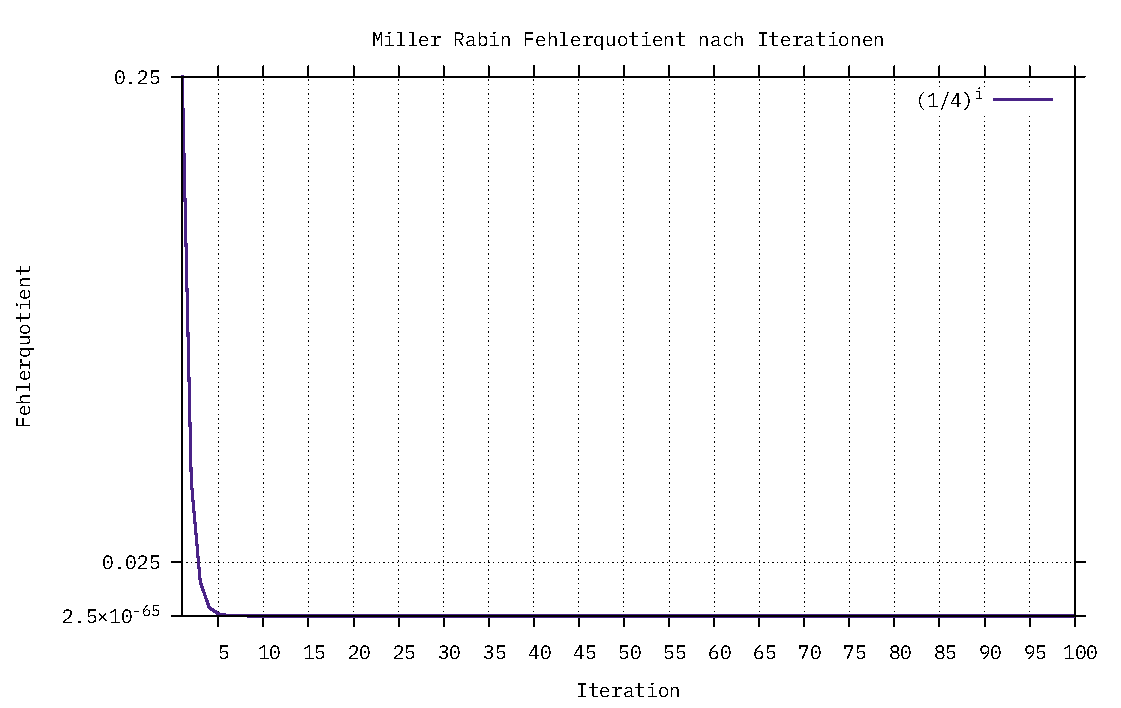
\includegraphics{mr_error.pdf}
  \label{mr_error}
  \caption{Fehlerquotient für $\left\{\,i \in \mathbb{N}\mid 1 \le i \le 100 \, \right\}$}
\end{figure}

\newpage

\subsubsection{Fermatscher Primzahltest}

Der kleine fermatsche Satz kann als rudimentärer Primzahltest verwendet werden, da die Kongruenz zwischen $a$ und $p$ nur gegeben ist, wenn $p$ eine Primzahl ist. Somit kann durch das iterative Testen dieser Kongruenz mit verschiedenen Basen $a$ ein Schluss auf die Primalität von $p$ gezogen werden:

\begin{figure}[h]
  \begin{cminted}

  // Falls die zu überprüfende Zahl 3 oder 2 ist
  if (n == 3 || n == 2)
    // Wahr zurückgeben
    return true;

  // Führe den Primzahltest für k Iterationen aus, beziehungsweise bis er fehlschlägt
  for (int _ = 0; _ < k; _++)
  {

    // Label zu dem gesprungen wird falls keine teilerfremde Base a gefunden werden konnte
    Restart:
                
    // Zufällige Base a mit 2 ≤ a ≤ n-2
    BigInteger a = GetRandomBigIntInRange(n.GetByteCount(), 2, n - 2);

    // Zählt die Anzahl der Versuche eine teilerfremde Base a basierend auf der selben Zufallszahl zu finden
    int coprimeRuns = 0;

    // Label zu dem gesprungen wird falls die derzeitige Base a nicht teilerfremd ist
    NotCoprime:

    // Falls die Base a mehr als 5 mal nicht teilerfremd war wird eine neue Zufallszahl generiert
    if (coprimeRuns > 5)
      goto Restart;

    // Untersuche ob a und n teilerfremd sind
    if (BigInteger.GreatestCommonDivisor(a, n) != 1)
    {
      // erhöhe die Base a um eins
      a++;
      // erhöhe die Anzahl der Versuche um eins
      coprimeRuns++;
      // springe zum vorherigen Label
      goto NotCoprime;
    }

    // Berechne a^n-1 mod n
    BigInteger res = ModPow(a, n - 1, n);

    // Falls der Rest nicht eins ist ist n nicht prim
    if (res != 1)
    {
      // Gebe falsch zurück
      return false;
    }
  }
  \end{cminted}
  \caption{Implementation eines Primzahltestes basierend auf dem kleinen fermatschen Satz}
\end{figure}

\newpage

\section{Eulersche Phi-Funktion}

Die Eulersche Phi-Funktion, auch bekannt als eulersche Totientfunktion, ist eine von Leonhard Euler 1763 formulierte Funktion der Zahlentheorie, welche die Summe der teilerfremden Zahlen zu $n$ darstellt\cite{pacific}:

\begin{equation}
  \begin{aligned}
    &n \in \mathbb{N}^+\\
    &\left\{\,\varphi(n) \in \mathbb{N}^+\mid 0 \le \varphi(n) \le n-1 \right\}\\
    &\varphi(n) = n \times \prod_{p\mid{}n}\left(1-\frac{1}{p}\right)
  \end{aligned}
\end{equation}

$\varphi(n)$ ist der Totient von $n$.

\begin{align}
  \varphi(5)&= 4 && \text{$\varphi(5) = n-1$, da n prim ist}\label{totative:1}\\
  \varphi(9)&= 6 && \text{teilerfremd zu $1_1$, $2_2$, $4_3$, $5_4$, $7_5$, $8_6$}\\
  \varphi(8)&= 4 && \text{teilerfremd zu $1_1$, $3_2$, $5_3$, $7_4$}\label{totative:2}\\ 
  \varphi(16)&= 8 && \text{teilerfremd zu $1_1$, $3_2$, $5_3$, $7_4$, $9_5$, $11_6$, $13_7$, $15_8$}\label{totative:3}
\end{align}

In Gleichungen \eqref{totative:1}, \eqref{totative:2} und \eqref{totative:3} sind zwei Spezialfälle für Werte $n$ der eulerschen Phi-Funktion zu sehen; Primzahlen und Potenzen zur Basis zwei:

\begin{enumerate}
  \item Für $n \in \mathbb{P}$ ist $\varphi(n)$ immer gleich $n-1$.\cite{mw02}
  \item Für $n=2^k \land k \ge 1$ ist $\varphi(2^k)=2^{k-1}$.
\end{enumerate}

Weitere Attribute der Funktion und ihrer Parameter sind:

\begin{enumerate}
  \item Für $n \ge 3$ ist $\varphi(n)$ immer  gerade, sprich $\varphi(n)=2k$.\cite{mw02}
  \item Konventionell ist $\varphi(0)=1$ definiert.\cite{mw02}
\end{enumerate}

Die eulersche Phi-Funktion findet auch Anwendung in einer Verallgemeinerung des kleinen fermatschen Satzes, welche von Euler auch 1763 publiziert wurde:

\begin{equation}
  a^{\varphi(n)} \equiv 1\pmod(n)
\end{equation}

Für alle Zahlen $a$ welche teilerfremd zu $n$ sind.\cite{mw03}

\ref{totative_dist} zeigt die Verteilung von $\varphi(n)$ für die ersten eintausend Werte $n$.

\begin{figure}[H]
  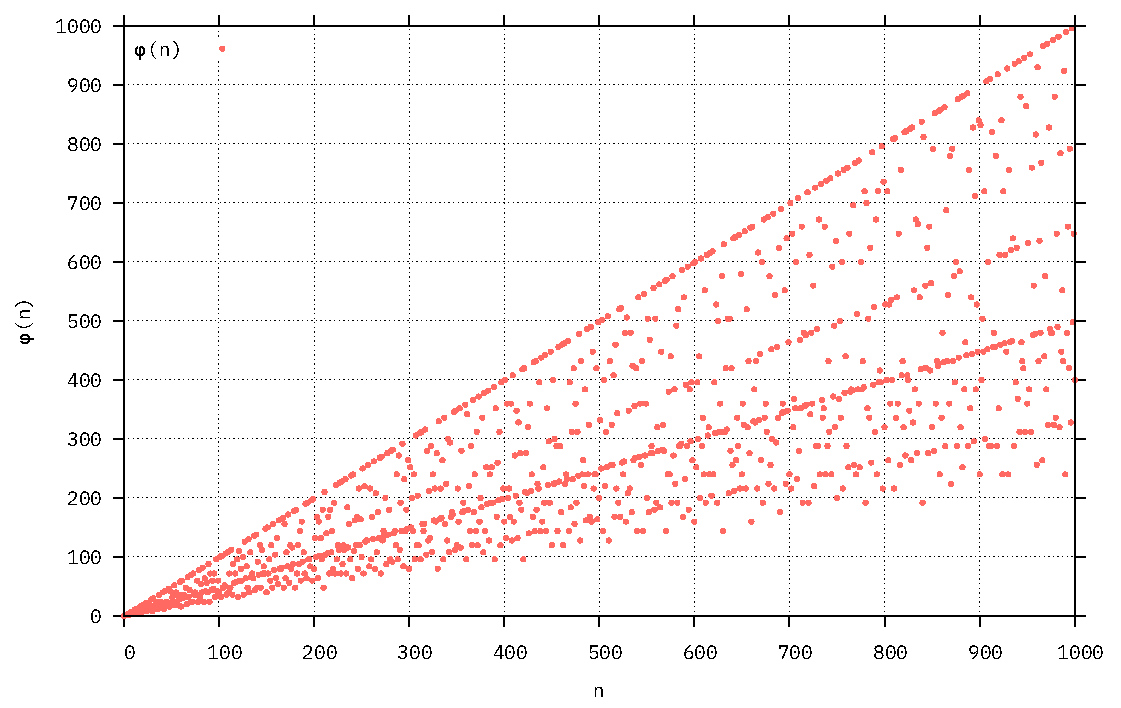
\includegraphics{totient.pdf}
  \caption{Eulersche Phi-Funktion $\varphi(n)$ für $\left\{\,n \in \mathbb{N}\mid 0 \le n \le 1000 \, \right\}$}
  \label{totative_dist}
\end{figure}

\newpage

\section{Carmichael-Funktion}

Die Carmichael-Funktion $\lambda(n)$ gibt für eine natürliche Zahl $n$ die kleinste positive ganze Zahl an, sodass für alle zu $n$ teilerfremden Zahlen $k$ gilt:

\begin{align}
  k^{\lambda(n)} \equiv 1\pmod{n}
\end{align}

Die Funktion kann wie folgt definiert werden:

\begin{align}
  \lambda(n) = \operatorname{kgV}\left[(p_i-1)p_i^{a_i-1}\right]_i
\end{align}\cite{mw04}

Hierbei steht $p_i$ für den i-ten Primfaktor von $n$ und $a_i$ für den Exponent des i-ten Primfaktores.\cite{mw05}

Um $\lambda(n)$ einer Zahl zu berechnen werden folgende Schritte verwendet:

\begin{enumerate}
  \item Zahl in Primfaktoren zerlegen
  \item Alle Primfaktoren in $(p_i-1)p_i^{a_i-1}$ einsetzen und die Ergebnisse speichern
  \item den kleinsten gemeinsamen Teiler aus allen Ergebnissen bilden
\end{enumerate}

Beispielhalft sei $n$ gleich $15$:

\begin{equation}
  \begin{aligned}
    n&=15=3^1 \cdot 5^1 && \text{Darstellung durch Primfaktoren}\\
    p_0&=3 && \text{Erster Primfaktor von $15$}\\
    p_1&=5 && \text{Zweiter Primfaktor von $15$}\\
    a_0&=1 && \text{Exponent des ersten Primfaktors $3$}\\
    a_1&=1 && \text{Exponent des zweiten Primfaktors $15$}\\
    k&=\left((p_0 - 1) \cdot p_0^{a_0 - 1};\, (p_1 - 1) \cdot p_1^{a_1 - 1}\right) && \text{Folge $k$ welche Ergebnisse enthält}\\
    \hookrightarrow&=\;\,((1;\, 12))\\
    \lambda(15)&=\operatorname{kgV}(k)=4
  \end{aligned}
\end{equation}

Oder für $n \in \mathbb{P}$:

\begin{equation}
  \begin{aligned}
    n&=17=17^1 && \text{Nur 1 und 17 als Primfaktor, da prim}\\
    p_0&=17\\
    a_0&=1\\
    k&=((17-1) \cdot 17^{1-1})\\
    \lambda(17)&=\operatorname{kgV}(k)=16
  \end{aligned}
  \label{carmichael:prime}
\end{equation}

die Berechnung in \ref{carmichael:prime} zeigt einen Sonderfall der Carmichael-Funktion, denn für alle $n \in \mathbb{P}$ ist $\lambda(n)=n-1$, wie in \ref{carmichael:primes} weiter zu sehen ist.

\begin{equation}
  \begin{aligned}
    \lambda(2)&=1\\
    \lambda(3)&=2\\
    \lambda(5)&=4\\
    \lambda(7)&=6\\
    \lambda(11)&=10\\
    \lambda(13)&=12\\
    ...&
  \end{aligned}
  \label{carmichael:primes}
\end{equation}

Abbildung \ref{carmichael_dist} zeigt die Verteilung von $\lambda(n)$ für die ersten eintausend Werte $n$. Abbildung \ref{carmichael_totient} zeigt eine kombinierte Verteilung von sowohl der eulerschen Phi-Funktion als auch der Carmichael-Funktion.

\begin{figure}[H]
  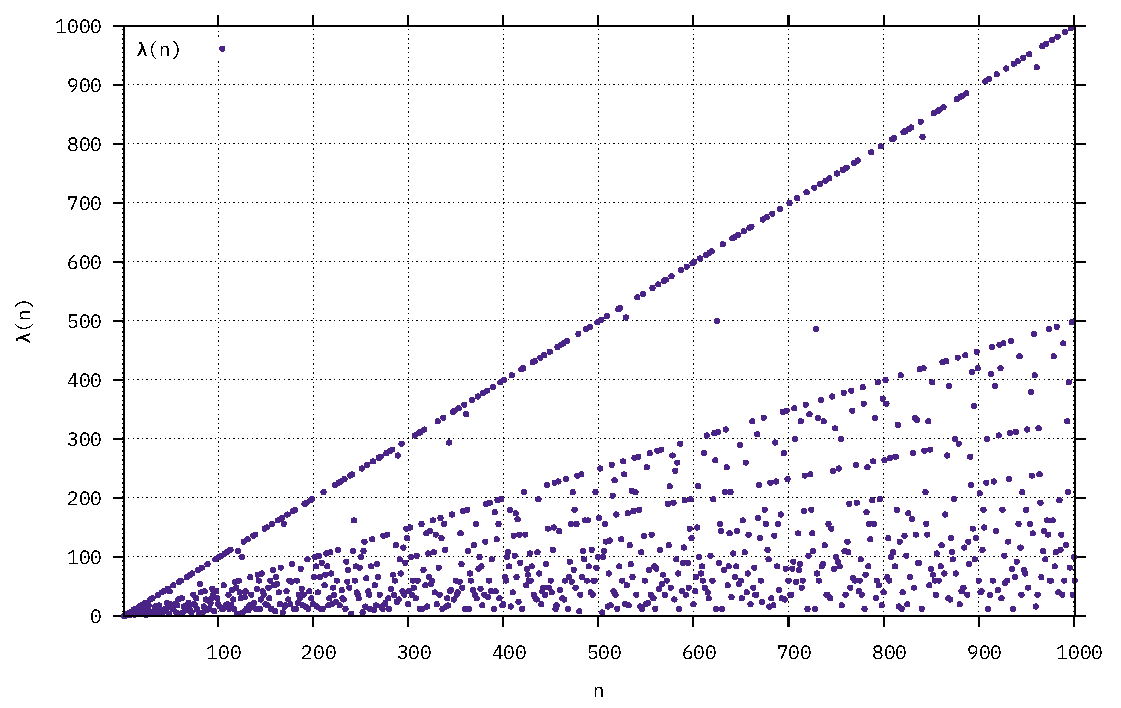
\includegraphics{carmichael.pdf}
  \caption{Carmichael-Funktion $\lambda(n)$ für $\left\{\,n \in \mathbb{N}\mid 1 \le n \le 1001 \, \right\}$}
  \label{carmichael_dist}
\end{figure}

\begin{figure}[H]
  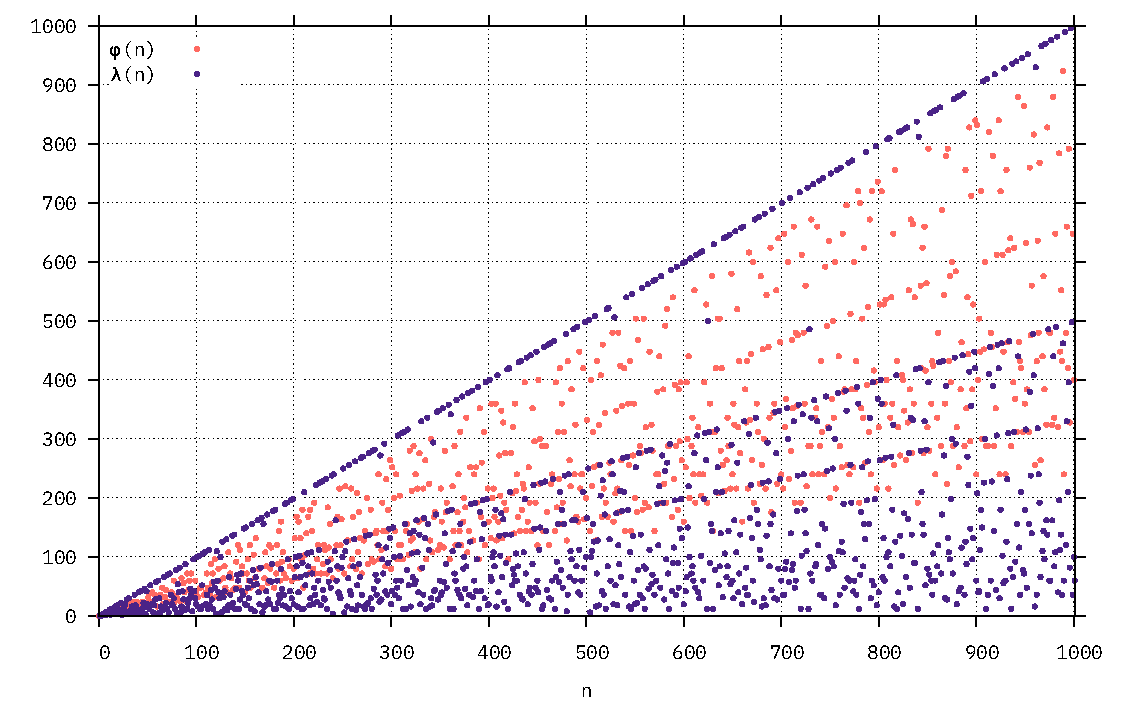
\includegraphics{totient_carmichael.pdf}
  \caption{Carmichael-Funktion $\lambda(n)$ für $\left\{\,n \in \mathbb{N}\mid 1 \le n \le 1001 \, \right\}$ und eulersche Phi-Funktion $\varphi(n)$ für $\left\{\,n \in \mathbb{N}\mid 0 \le n \le 1000 \, \right\}$}
  \label{carmichael_totient}
\end{figure}

\newpage

\section{Euklidischer Algorithmus}
A.
\subsection{Erweiterter Euklidischer Algorithmus}

\newpage

\section{Chinesischer Restsatz}
